\documentclass{article}
\usepackage{tikz}
\usetikzlibrary{decorations}
\title{Shapes}
\author{Pritha}

\begin{document}
	\maketitle
	\tableofcontents
	\clearpage
	
	\section{Lines}
	\vspace{1cm}
		\subsection{Straight Line}
			\begin{center}
				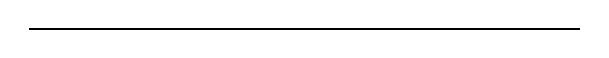
\begin{tikzpicture}
					\draw[thick] (0, 0) -- (7, 0);
				\end{tikzpicture}
			\end{center}
			
		\subsection{Directed Line}
			\begin{center}
				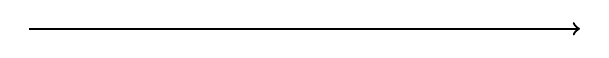
\begin{tikzpicture}
					\draw[thick, ->] (0, 0) -- (7, 0);
				\end{tikzpicture}
			\end{center}
						
		\subsection{Axes Lines}
		%\vspace{1cm}
			\begin{center}
				\begin{tikzpicture}
					\draw[thick, ->] (0, 0) -- (4, 0) node[anchor = north west]{x axis};
					\draw[thick, ->] (0, 0) -- (0, 4) node[anchor = south east] {y axis};
				\end{tikzpicture}
			\end{center}
			
		\subsection{Curved Line}
			\begin{center}
				\begin{tikzpicture}
					\draw[thick] (0, 0) ..controls (0, 2) and (4, 0) .. (4, 4);
				\end{tikzpicture}
			\end{center}
			
			
	\section{Circles}
	\vspace{1cm}
		\subsection{Circle}
			\begin{center}				
				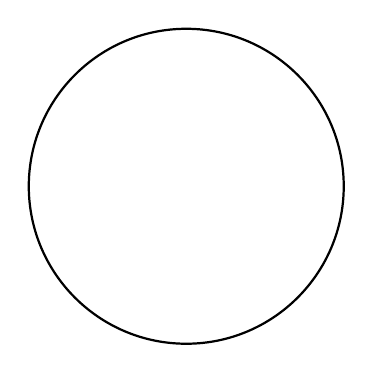
\begin{tikzpicture}
					\draw[thick] (0, 0) circle (2);
				\end{tikzpicture}
			\end{center}
			
		\subsection{Dashed Circle}
			\begin{center}				
				\begin{tikzpicture}
					\draw[thick, red, dashed] (0, 0) circle (2);
				\end{tikzpicture}
			\end{center}
			
		\subsection{Dashed and Dotted Circle}
			\begin{center}				
				\begin{tikzpicture}
					\draw[thick, blue, dash dot] (0, 0) circle (2);
				\end{tikzpicture}
			\end{center}
	
	
	\section{Triangle}
	\vspace{1cm}
		\begin{center}
			\begin{tikzpicture}
				\draw (0, 0) -- (3, 0);							\draw (0, 0) -- (0, 3);
				\draw (3, 0) -- (0, 3);
			\end{tikzpicture}
		\end{center}
		
		
	\section{Rectangle}
	\vspace{1cm}
		\begin{center}
			\begin{tikzpicture}
				\draw (0, 0) rectangle (2, 2);
			\end{tikzpicture}
		\end{center}
		
		
	\section{Parabolas}
	\vspace{1cm}
		\subsection{Half a Parabola}
			\begin{center}
				\begin{tikzpicture}
					\draw (0, 0) parabola (2, 2);
				\end{tikzpicture}
			\end{center}
			
		\subsection{Parabola}
			\begin{center}
				\begin{tikzpicture}
					\draw[thick, domain=-2:2, samples=100] plot (\x, {\x*\x});
				\end{tikzpicture}
			\end{center}
			
			
	\section{Grid}
	\vspace{1cm}
		\begin{center}
				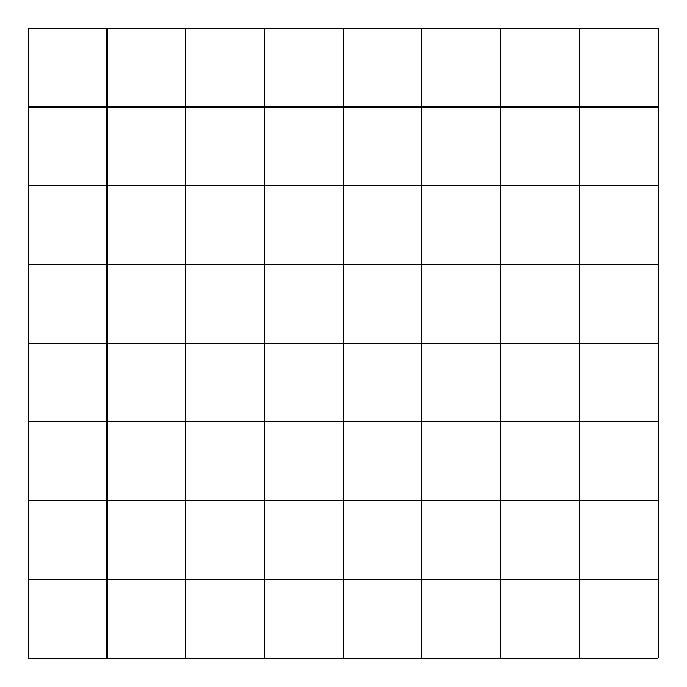
\begin{tikzpicture}
					\draw[step = 1cm, black, thin](-2, -2) grid (6,6);
				\end{tikzpicture}
			\end{center}
			
			
	\section{Arc}
	\vspace{1cm}
		\begin{center}
				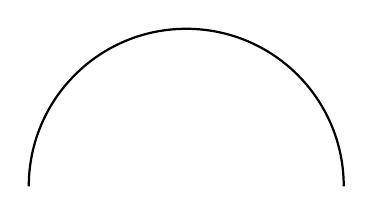
\begin{tikzpicture}
					\draw[thick](0, 0) arc (0:180:2cm);
				\end{tikzpicture}
			\end{center}
			
			
	\section{Ellipse}
	\vspace{1cm}
		\begin{center}
				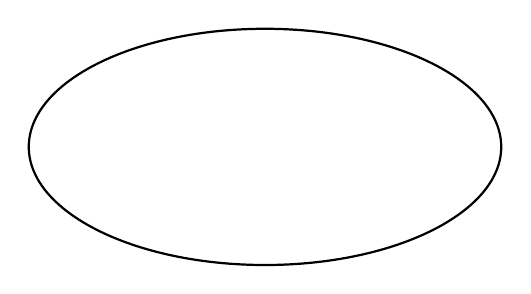
\begin{tikzpicture}
					\draw[thick](0, 0) ellipse (3cm and 1.5cm);
				\end{tikzpicture}
			\end{center}
			
	\newpage	
	\section{Practice}
	\vspace{1cm}
		\begin{center}
			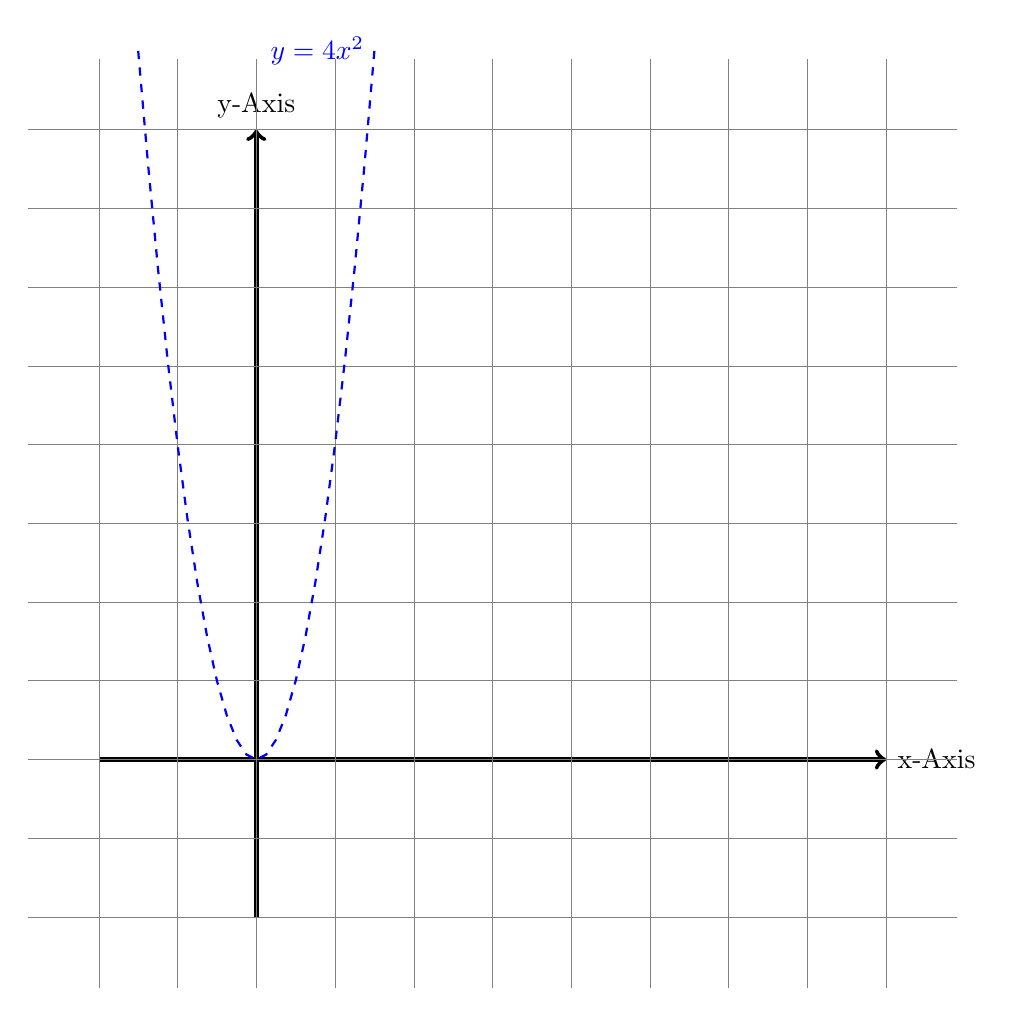
\begin{tikzpicture}
				\draw[<-,->,ultra thick](-2,0)--(8,0)node[right]{x-Axis};
				\draw[<-,->,ultra thick](0,-2)--(0,8)node[above]{y-Axis};
				\draw[gray, very thin](-2.9,-2.9) grid (8.9,8.9);
				\draw[domain = -1.5:1.5, thick, blue, dashed] plot(\x,{4*\x*\x}) node [left]{$y=4x^2$};
			\end{tikzpicture}
		\end{center}
\end{document}